% \appendix
\renewcommand{\thechapter}{A}
\chapter{Usage of AlgTest pyProcess}

\definecolor{codegreen}{rgb}{0,0.6,0}
\definecolor{codegray}{rgb}{0.5,0.5,0.5}
\definecolor{codepurple}{rgb}{0.58,0,0.82}
\definecolor{backcolour}{rgb}{0.95,0.95,0.92}

\lstdefinestyle{mystyle}{
    backgroundcolor=\color{white},   
    commentstyle=\color{codegreen},
    keywordstyle=\color{magenta},
    numberstyle=\tiny\color{codegray},
    stringstyle=\color{codepurple},
    basicstyle=\ttfamily\footnotesize,
    breakatwhitespace=false,         
    breaklines=true,                 
    captionpos=b,                    
    keepspaces=true,                          
    showspaces=false,                
    showstringspaces=false,
    showtabs=false,                  
    tabsize=2
}

\lstset{style=mystyle}

\section{Installation}
After cloning into repository containing \texttt{AlgTest process} tool, it is necessary to install a few dependencies. The project includes a script called \texttt{setup.py} which, when ran installs required packages. It may be convenient to create a Python virtual environment that allows us to install and manage Python project packages locally without unnecessary global installation. It is important to create and source a virtual environment before running the setup script.
\begin{lstlisting}[language=bash]
    $ python -m venv venv
    $ source venv/bin/activate
    $ python setup.py
\end{lstlisting}

\section{Folder structure}
\begin{itemize}
    \item \texttt{algtestprocess}
        \begin{itemize}
            \item \texttt{modules} -- folder containing \texttt{algtestprocess} modules.
                \begin{itemize}
                    \item \texttt{components} -- folder containing reusable code for parts of HTML documents. Each file contains classes, constants related to one component.
                    \item \texttt{pages} -- folder containing files with classes corresponding to generated HTML pages, each page has a separate file containing class which is responsible for page creation.
                    \item \texttt{parser}
                        \begin{itemize}
                            \item \texttt{javacard} -- folder containing parser implementations for JavaCard profiles
                            \item \texttt{tpm} -- folder containing parser implementations for TPM profiles
                        \end{itemize}
                    \item \texttt{config.py} -- file containing classes for choice of algorithms used in specific pages
                    \item \texttt{jcalgtest.py} -- file containing classes for storage of Java Card profiles
                    \item \texttt{tpmalgtest.py} -- file containing classes for storage of TPM profiles
                \end{itemize}
        \end{itemize}
    \item \texttt{setup.py} -- script for installation of dependencies and download of results from their official GitHub repository\footnote{\url{https://github.com/crocs-muni/jcalgtest_results}}
    \item \texttt{process.py} -- main entrypoint for generation of outputs, its usage is described in following section
\end{itemize}

\section{Usage}
The script process.py provides a CLI in the following way:

\begin{itemize}
    \item Set of operations from \texttt{process, all, execution-time, comparative, radar, scalability, similarity, support}. We can select multiple operations; however, \texttt{process} operation needs to be run at least once so that some issues with CSV files are fixed, and JSON outputs are generated for the following operations which use them. In the subsequent runs the \texttt{process} argument is not necessary.
    \item \texttt{-i/-{}-results-dir} A directory with measurement results.
    \item \texttt{-o/-{}-output-dir} Output directory to which the HTML outputs are stored.
\end{itemize}

\begin{lstlisting}[language=bash]
    $ python process.py process all --results-dir ./jcalgtest_results/ --output-dir ./jcalgtest_results/javacard/web
    $ python process.py radar scalability -i ./jcalgtest_results/ -o ./jcalgtest_results/javacard/web
\end{lstlisting}

\renewcommand{\thechapter}{B}
\chapter{Diagrams and Visualizations}\label{appendix:diagrams-visualizations}

\begin{figure}[H]
    \centering
    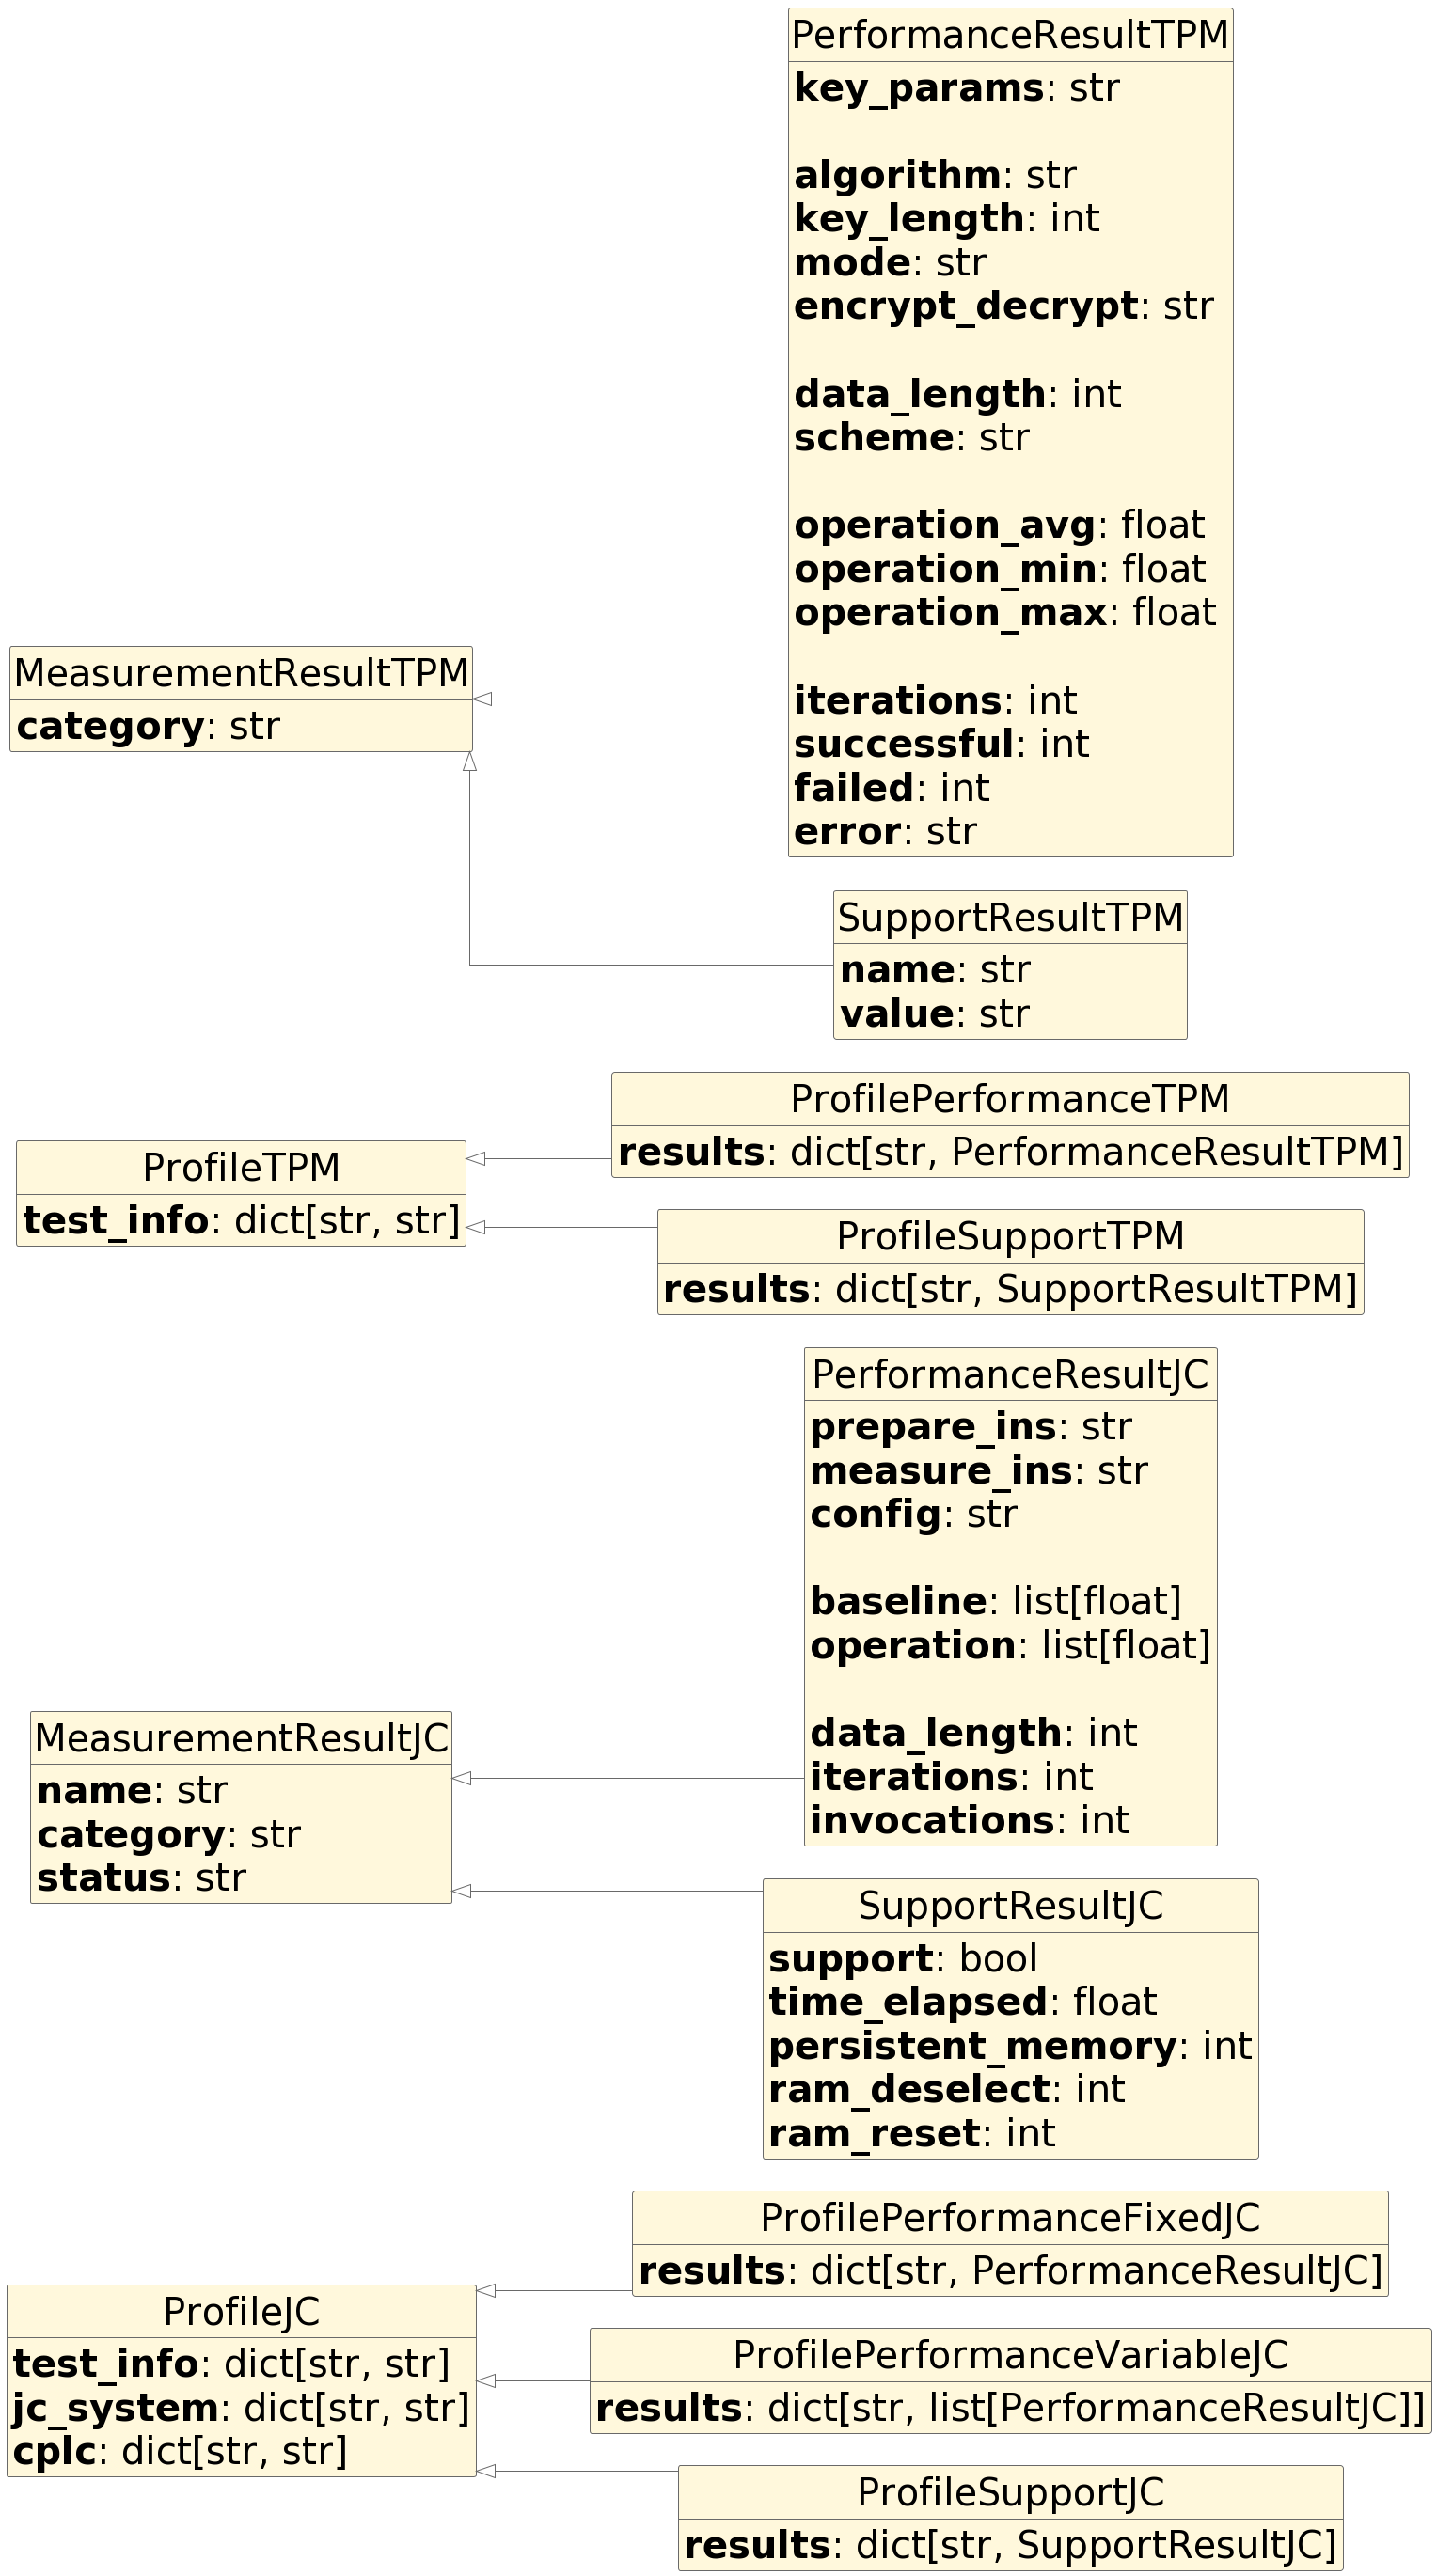
\includegraphics[width=\textwidth,height=\textheight-4.5cm, keepaspectratio]{img/diagrams/object_diagram.png}
    \caption{Diagram of Device profiles}
    \label{fig:dev-profiles-diagram}
\end{figure}

\begin{landscape}
    \begin{figure}[!t]
        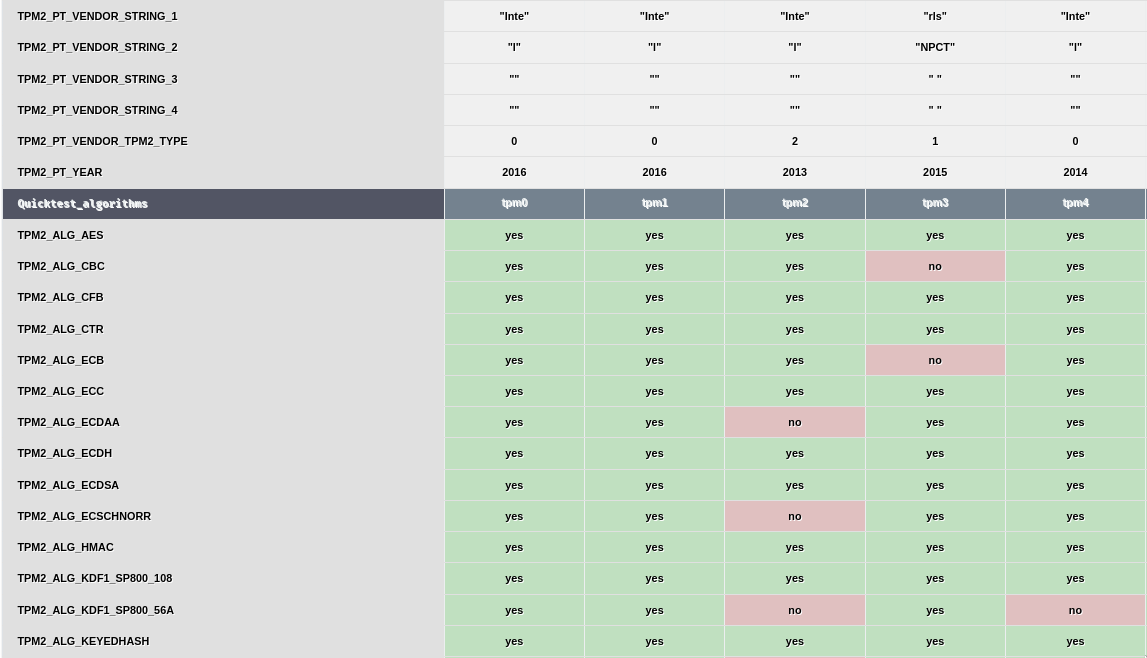
\includegraphics[width=\linewidth, height=\textwidth]{img/visualizations/tpm-support-data.png}
        \caption{An example of a part of Support table visualization for the TPMs}
    \end{figure}
\end{landscape}

\begin{landscape}
    \begin{figure}[!t]
        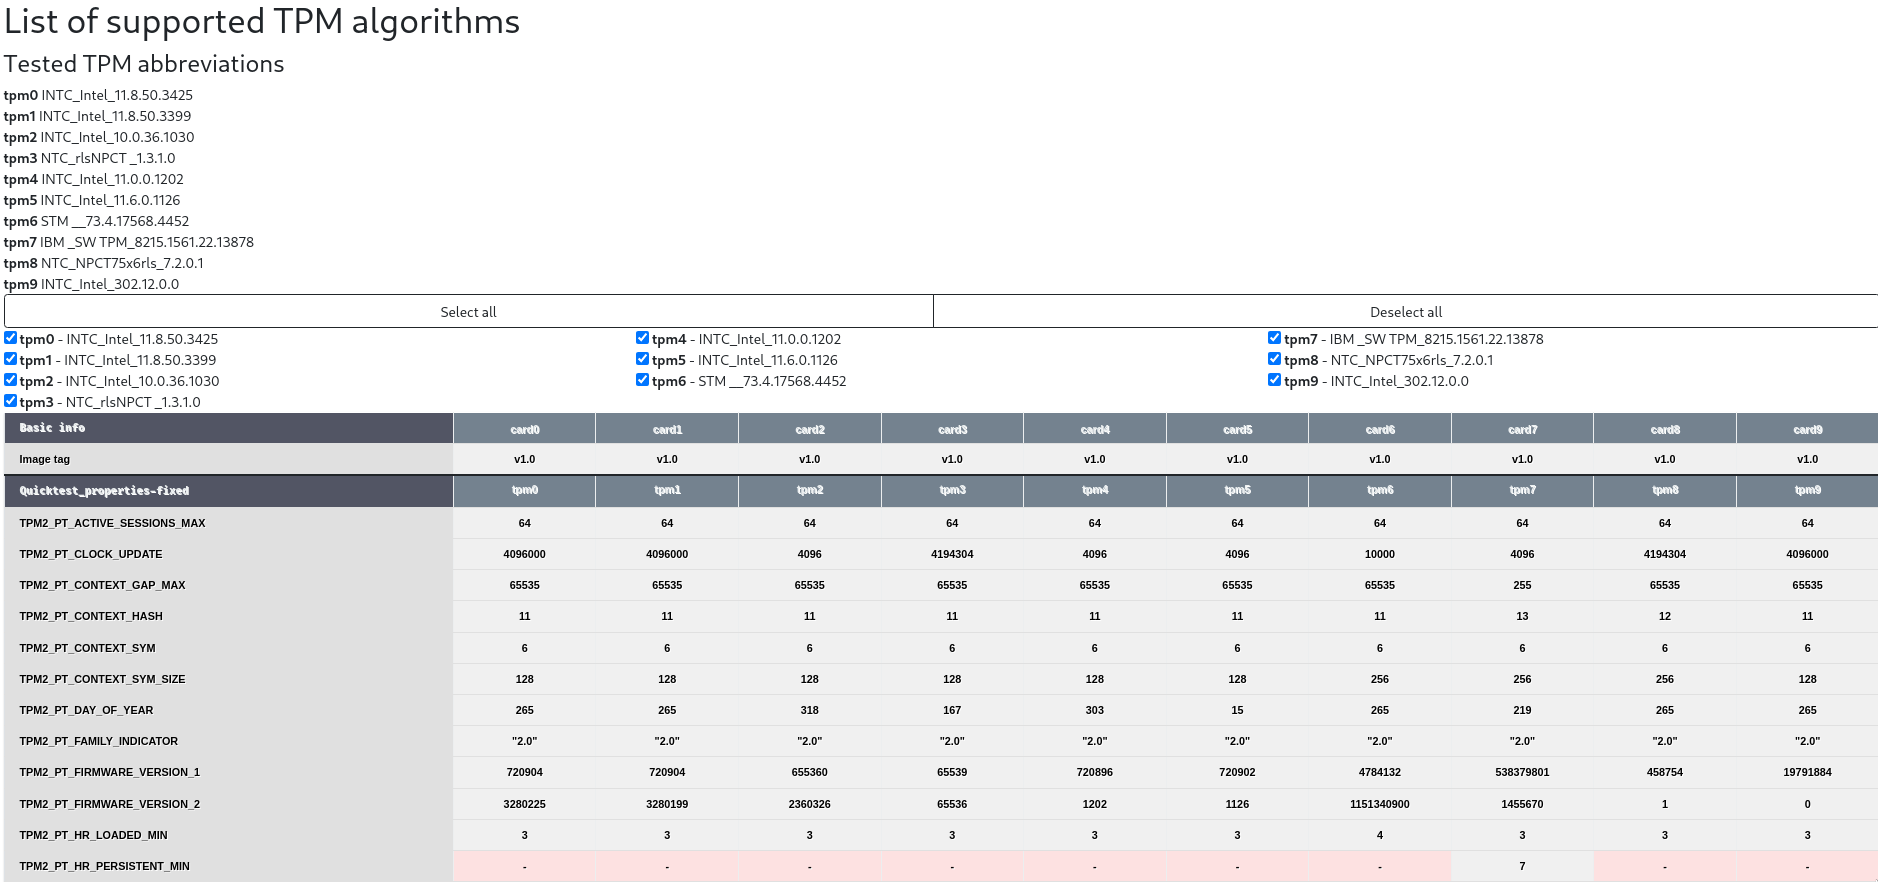
\includegraphics[width=\linewidth, height=\textwidth]{img/visualizations/tpm-support-utility.png}
        \caption{Support tables also contain checkbox utility for filtering the devices}
    \end{figure}
\end{landscape}

\begin{landscape}
    \begin{figure}[!t]
        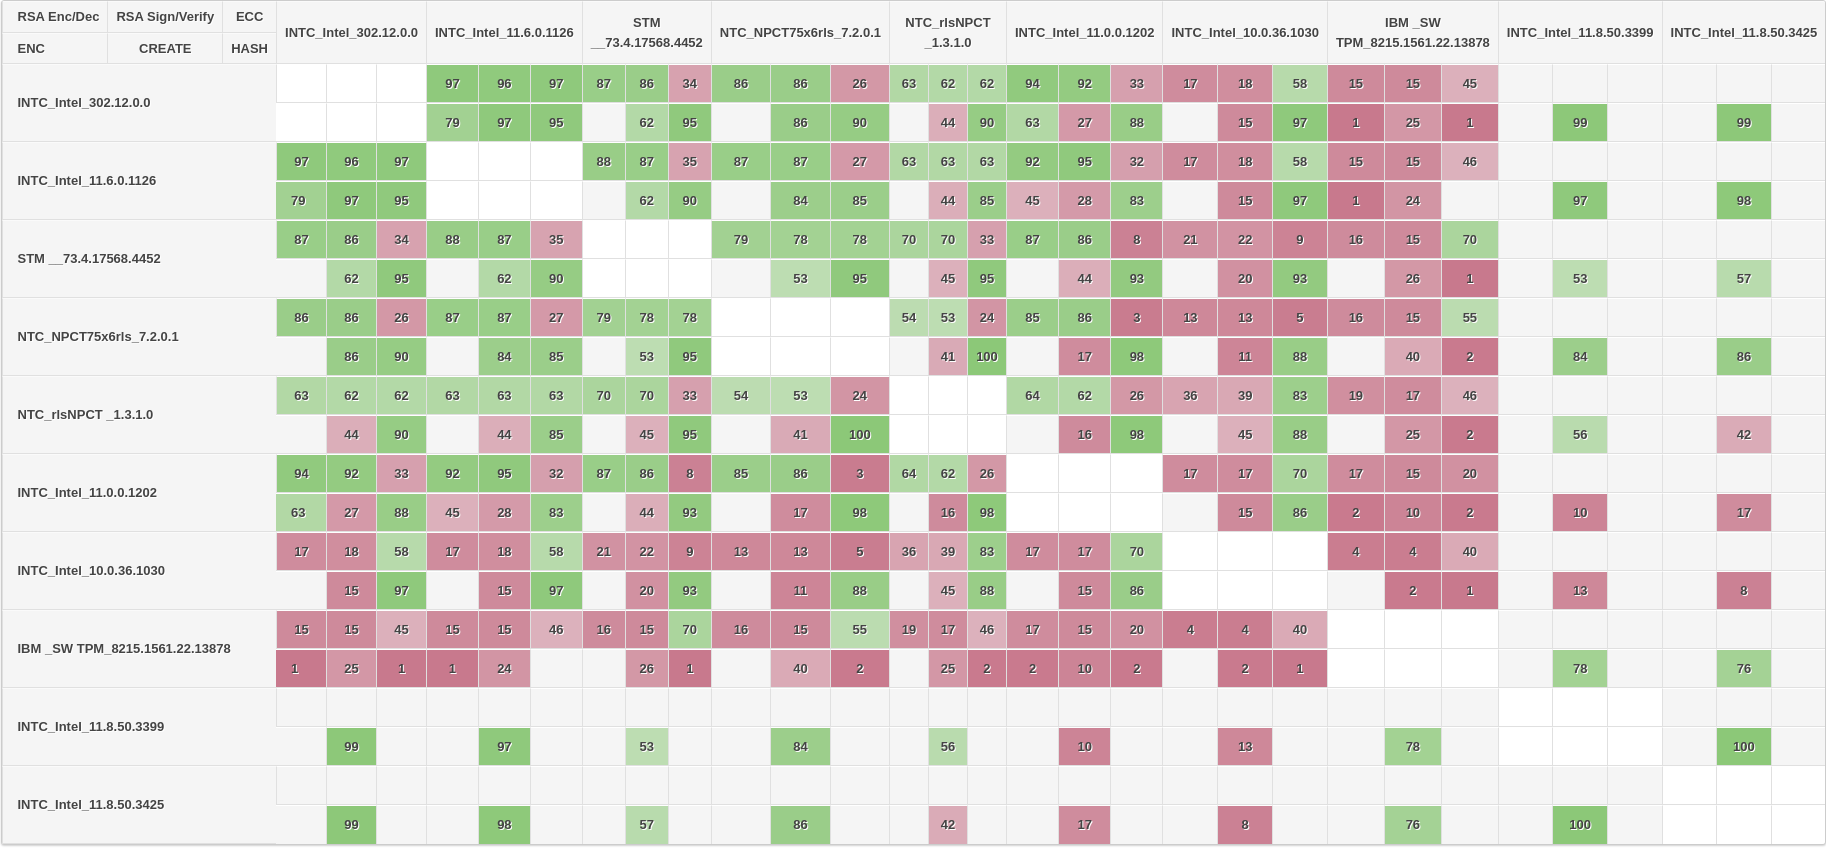
\includegraphics[width=\linewidth, height=\textwidth]{img/visualizations/tpm-similarity.png}
        \caption{Similarity table for TPMs}
    \end{figure}
\end{landscape}

\begin{landscape}
\begin{figure}[!t]
    \centering
    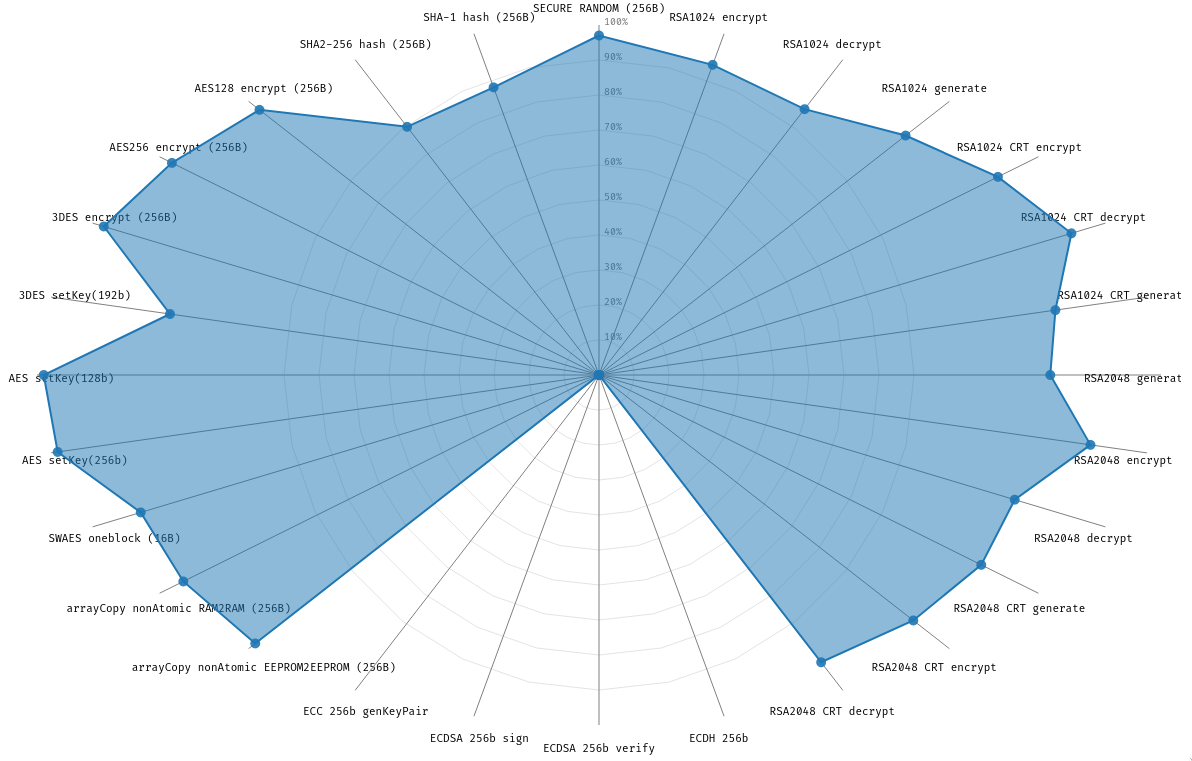
\includegraphics[width=\linewidth]{img/visualizations/JC30M48CR radar graph.png}
    \caption{
    The radar graph of the JC30M48CR smart card. Its performance can be considered excellent, apart from no evident support for algorithms involving Elliptic Curve Cryptography signified by a cut-out at the bottom of the graph.
    }
\end{figure}
\end{landscape}

\begin{landscape}
\begin{figure}[!t]
    \centering
    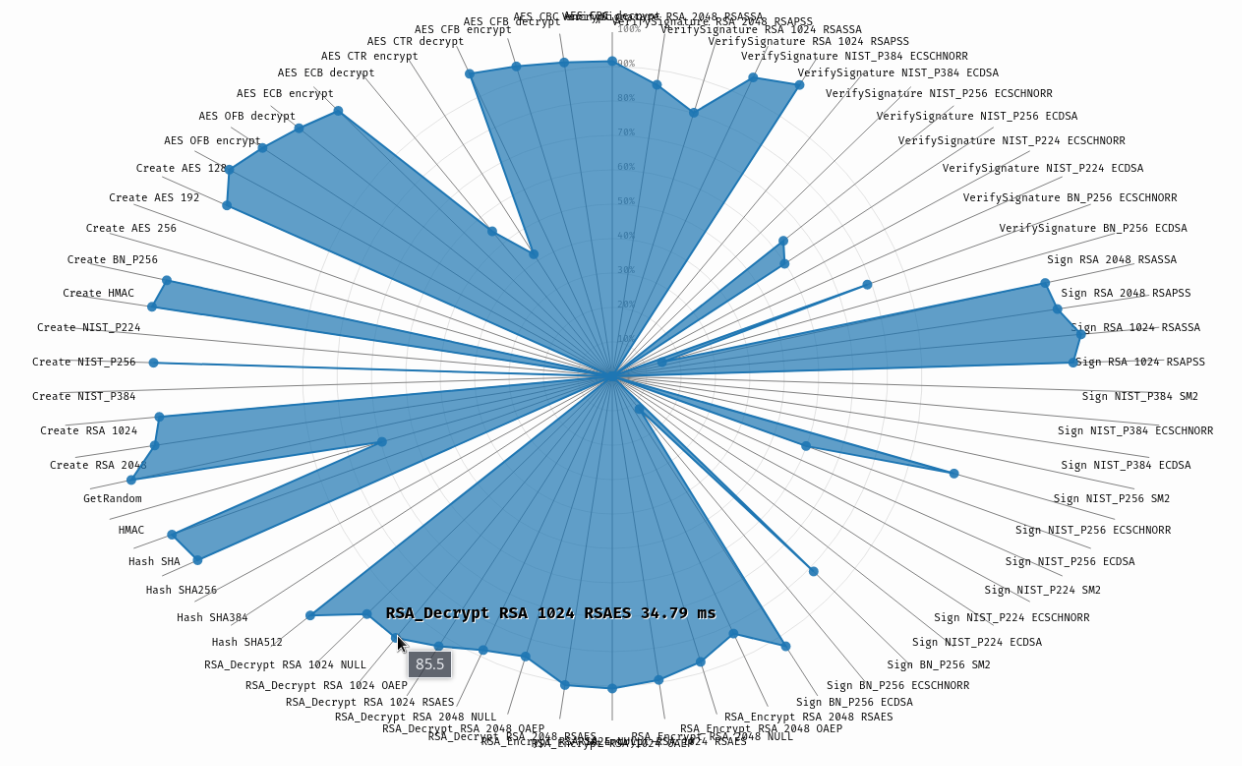
\includegraphics[width=\linewidth]{img/visualizations/INTC_Intel_302.12.0.0 radar graph.png}
    \caption{
    The radar graph of the INTC Intel 302.12.0.0 TPM.
    }
\end{figure}
\end{landscape}
\begin{figure}[H]
    \centering
    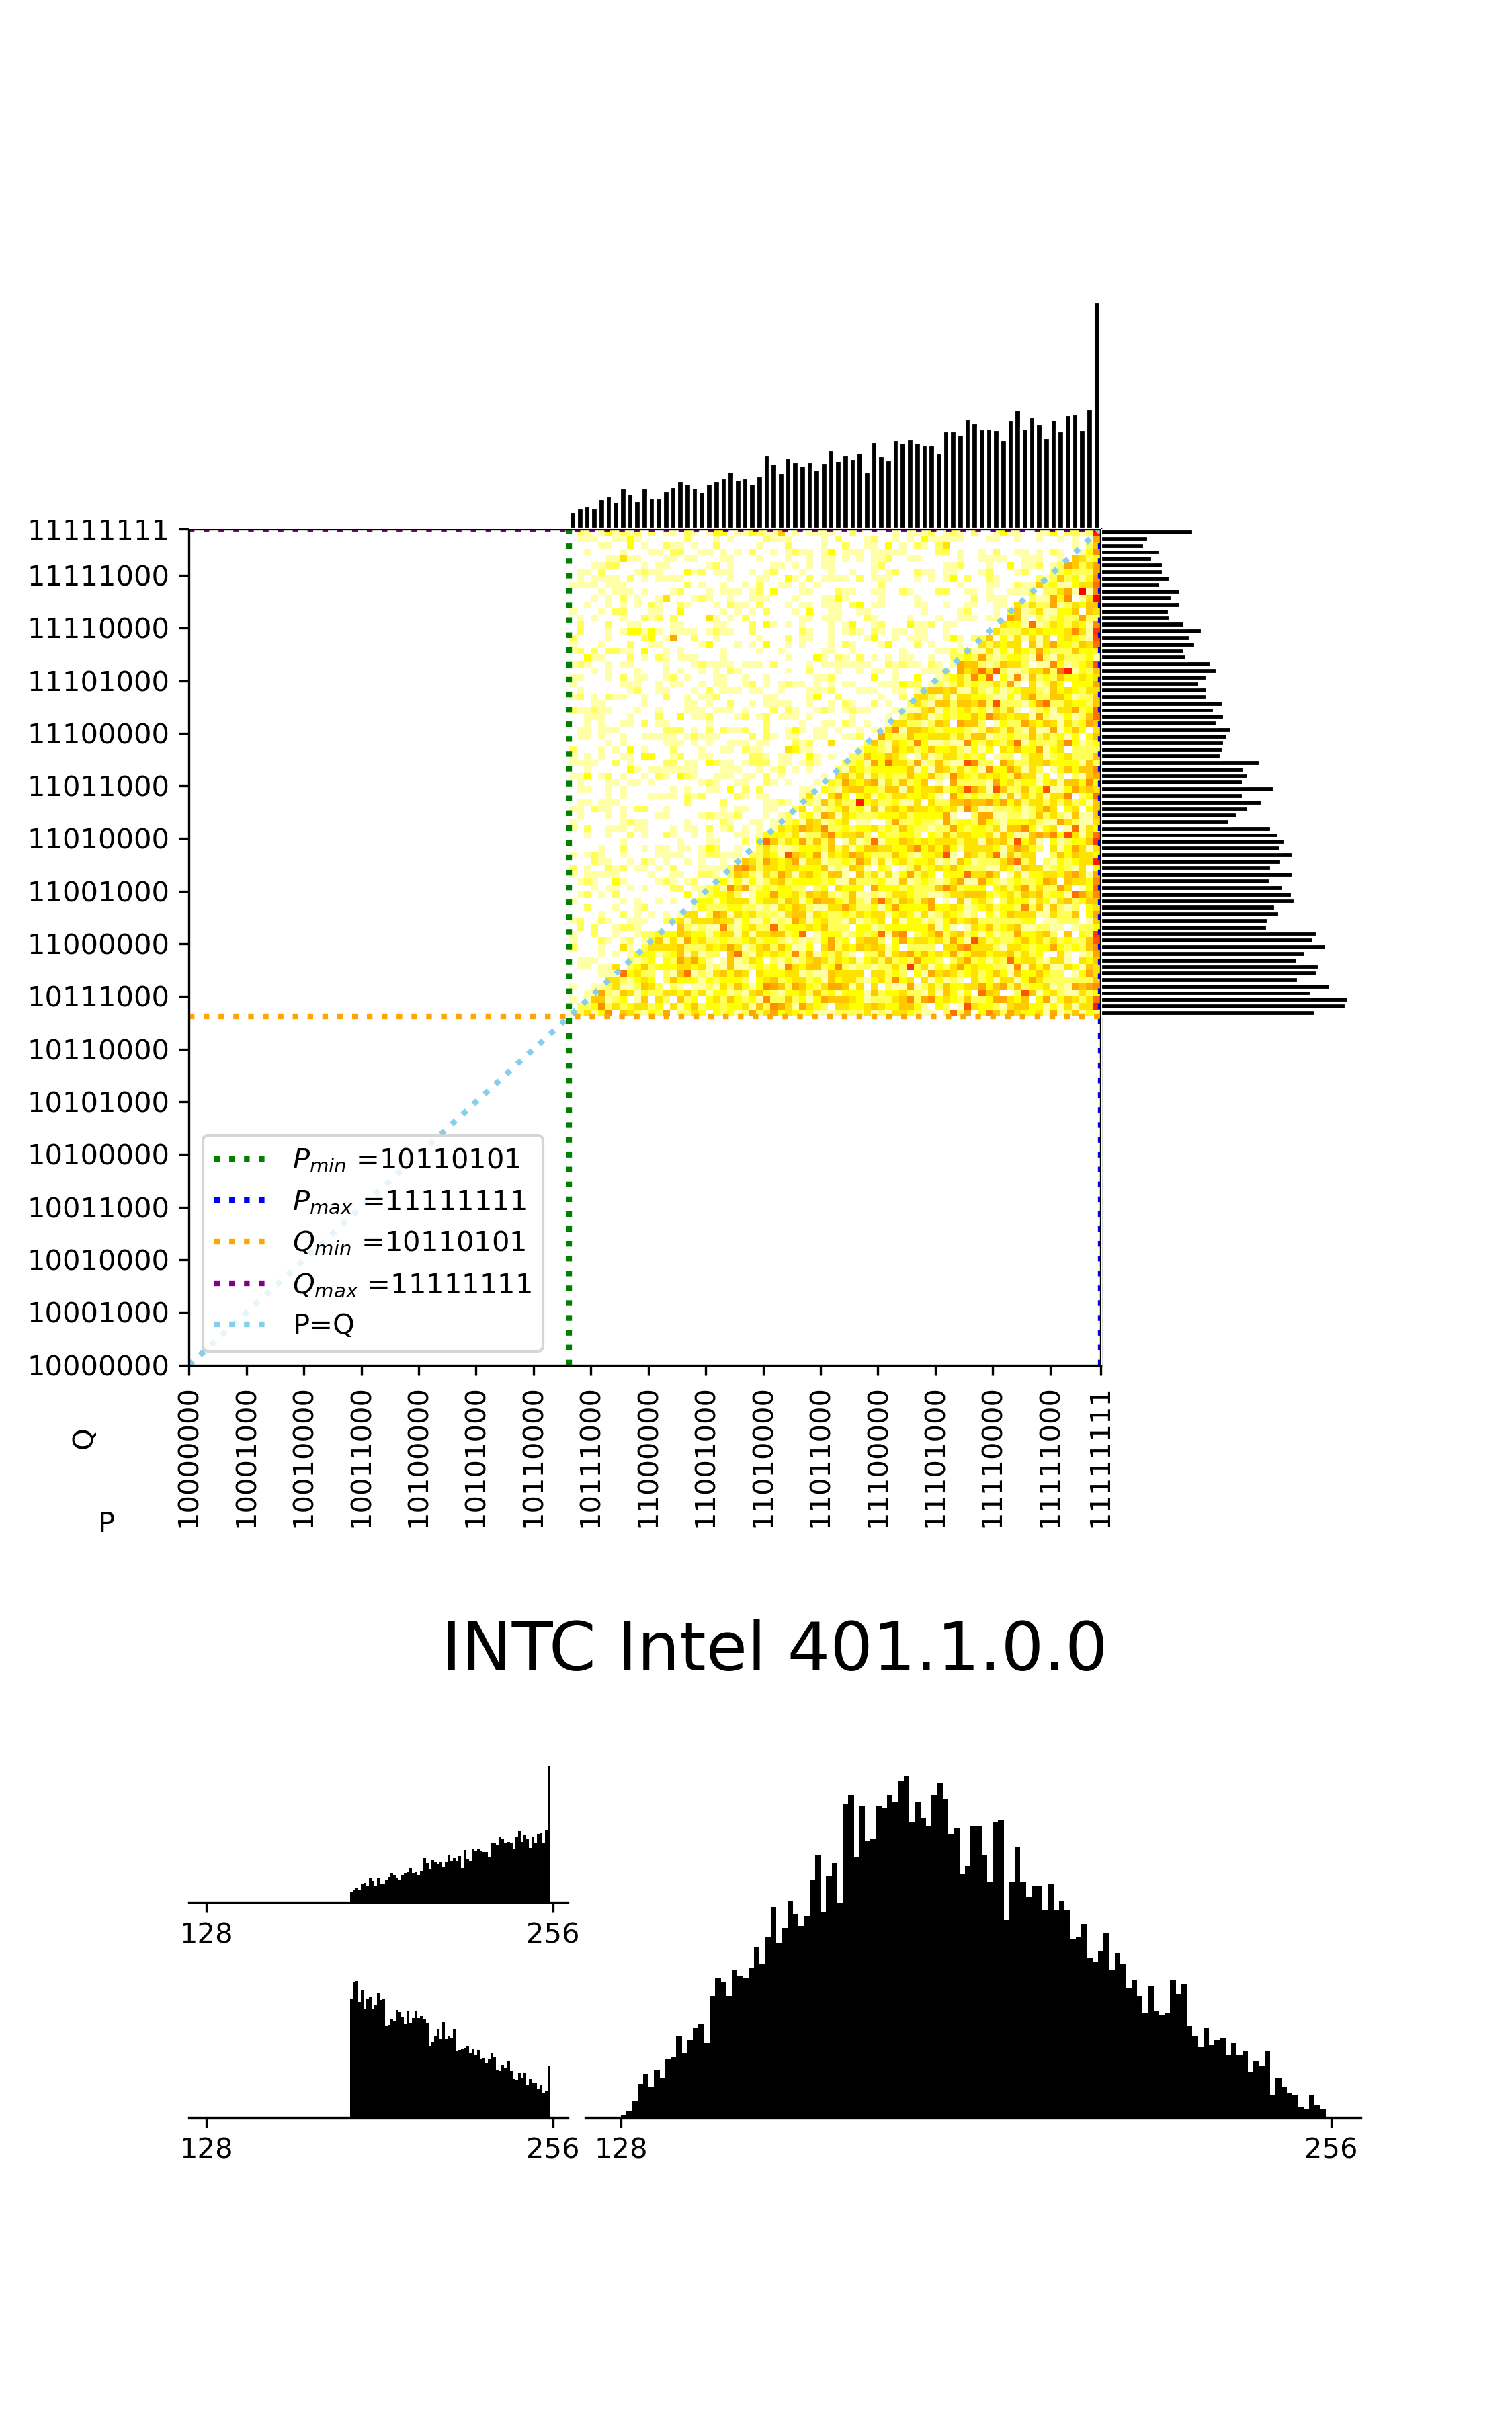
\includegraphics[width=\textwidth,height=\textheight-1.5cm, keepaspectratio]{img/visualizations/rsa.png}
    \caption{TPM chart showing the heatmap and several histograms of most significant bytes of gathered 1024 bit RSA keys.}
    \label{fig:dev-profiles-diagram}
\end{figure}





\renewcommand{\thechapter}{C}
\chapter{Data Attachments}